\section{可测输入}
\label{sec:ivp-measurable}

前面的结论都假设右端连续。实际的输入常常不连续：开关切换，继电器动作，信号被采样后保持。这时曲线在切换时刻不可能处处满足方程，解又该怎样定义？积分形式给出答案。

\paragraph{一次切换}
一个房间的温度偏差$x$满足$\dot{x}=-x+g(t)$，$x(0)=0$，暖气的作用是
\[
 g(t)=\begin{cases}1,&0\leq t<1,\\0,&t\geq 1.\end{cases}
\]
在$[0,1)$上$g\equiv 1$，这是冷却方程~\eqref{eq:ivp-cooling}的情形（$k=1$，$c=1$），由式~\eqref{eq:ivp-cooling-solution}，
\[
 x(t)=1-\mathrm{e}^{-t},\qquad 0\leq t\leq 1.
\]
温度不会突变，所以第二段以$x(1)=1-\mathrm{e}^{-1}\approx 0.632$为初值。在$t\geq 1$上$\dot{x}=-x$，因此
\[
 x(t)=(1-\mathrm{e}^{-1})\,\mathrm{e}^{-(t-1)},\qquad t\geq 1.
\]

\begin{BookInlineFigure}
 \centering
 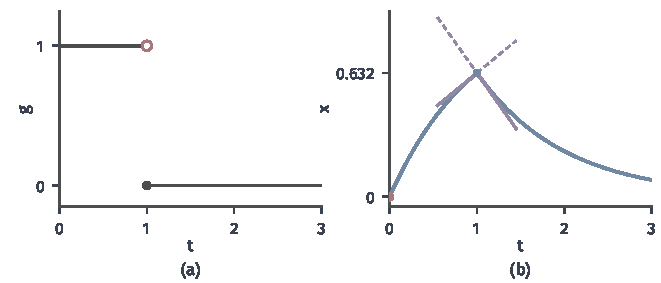
\includegraphics[width=112mm]{figures/06-differential-equations/01-ordinary-differential-equations/matplotlib/ivp-switching-input/figure.pdf}
 \caption{一次切换。(a)输入$g$在$t=1$从$1$跳到$0$。(b)解在$t=1$处连续但有折角。紫色实线是左右两侧的切线，斜率分别为$\mathrm{e}^{-1}\approx 0.368$和$-0.632$，紫色虚线是它们的延长。}
 \label{fig:ivp-switching-input}
\end{BookInlineFigure}

图~\ref{fig:ivp-switching-input}(b)的曲线在$t=1$连续，但左右导数不同：
\[
 \dot{x}(1^{-})=-0.632+1=0.368,\qquad\dot{x}(1^{+})=-0.632.
\]
这样的曲线在$t=1$不可微，不是定义~\ref{def:ivp-classical-solution}意义下的解，并且无论把$g(1)$规定成什么都不可能是。把两段分别解出来再接起来，所得的曲线却是唯一合理的答案。它的一个重要性质是满足积分方程：对$t\leq 1$，
\[
 \int_0^t(-x(s)+1)\,\mathrm{d}s=\int_0^t\mathrm{e}^{-s}\,\mathrm{d}s=1-\mathrm{e}^{-t}=x(t).
\]
对$t>1$，把积分在$1$处分开，后一段被积函数是$-x(s)$，由此验证
\[
 x(1)+\int_1^t(-x(s))\,\mathrm{d}s
 =x(1)+x(1)\bigl(\mathrm{e}^{-(t-1)}-1\bigr)=x(t).
\]
积分不在乎被积函数在一个点上的取值，所以$g(1)$取$0$或$1$都不影响。这启发我们用积分方程作为解的定义。

\paragraph{切换无穷多次}
有限次切换总可以分段解决。但输入可能更不规则。图~\ref{fig:ivp-irregular-inputs}给出两种情形，方程都取$\dot{x}=g(t)$，$x(0)=0$，所以解就是$g$的累积。

第一种，$g(t)=\operatorname{sign}\sin(1/t)$，$t\in(0,1]$。切换点$1/(k\pi)$在$t=0$附近聚集，无法从起点开始分段：不存在“第一段”。

第二种，$g$是胖Cantor集$C\subset[0,1]$的指示函数。构造方法是：第$k$步从剩下的每段中间挖去长度$4^{-k}$的开区间，极限集合$C$是闭集，不含任何区间，总长度却是$1-\sum_{k\geq 1}2^{k-1}4^{-k}=1/2$。$g$在$C$的每一点都不连续，而这些点的总长度为正，所以$g$不是Riemann可积的，分段的办法和连续函数的积分都不适用。

\begin{BookInlineFigure}
 \centering
 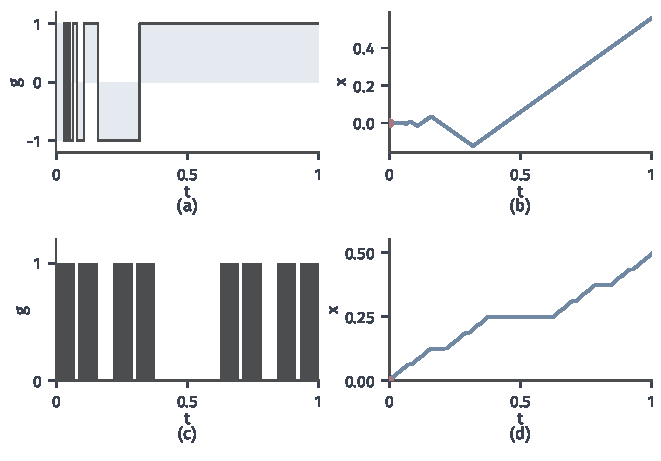
\includegraphics[width=112mm]{figures/06-differential-equations/01-ordinary-differential-equations/matplotlib/ivp-irregular-inputs/figure.pdf}
 \caption{不能分段处理的输入，方程为$\dot{x}=g$，$x(0)=0$。(a)$g=\operatorname{sign}\sin(1/t)$，切换点向$t=0$聚集（$t<0.03$只画出浅色填充）。(b)它的累积。(c)胖Cantor集的指示函数（挖到第$11$层的近似）。(d)它的累积$x(t)$是$[0,t]$中集合$C$的长度，$x(1)=1/2$。}
 \label{fig:ivp-irregular-inputs}
\end{BookInlineFigure}

两种情形中$g$都是有界可测函数，Lebesgue积分有意义，累积$x(t)=\int_0^t g$是连续曲线。这两条累积曲线都不能分成有限段来求，却也都由输入唯一确定，解的概念应当能容纳它们。

\paragraph{为什么要绝对连续}
一个自然的想法是放宽为“连续，并且几乎处处满足方程”。这不够。考虑$\dot{x}=0$，$x(0)=0$，Cantor函数$c:[0,1]\to[0,1]$满足$c(0)=0$，它连续，在Cantor集之外导数为零，而Cantor集长度为零，所以它几乎处处满足方程。可是$c(1)=1$，它一路上升了，而方程说的是不变。图~\ref{fig:ivp-cantor-candidate}中的红线就是这样的假解。

\begin{BookInlineFigure}
 \centering
 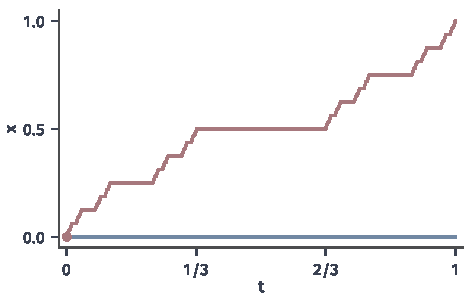
\includegraphics[width=80mm]{figures/06-differential-equations/01-ordinary-differential-equations/matplotlib/ivp-cantor-candidate/figure.pdf}
 \caption{方程$\dot{x}=0$，$x(0)=0$的解是蓝线$x\equiv 0$。红线是Cantor函数，连续且几乎处处导数为零，却从$0$升到$1$，不满足积分方程$x(t)=0+\int_0^t0\,\mathrm{d}s$。}
 \label{fig:ivp-cantor-candidate}
\end{BookInlineFigure}

Cantor函数的全部增长都发生在一个长度为零的集合上，导数看不见它，所以累积不回去。我们需要的正是“增量可以由导数累积回来”的函数，这恰是绝对连续函数的特征。区间$[a,b]$上的函数$F$称为\term{绝对连续函数}，是指对任意$\varepsilon>0$，存在$\delta>0$，使总长度小于$\delta$的有限个不交子区间上的增量绝对值之和小于$\varepsilon$。

这个定义恰好对应一种形式的微积分基本定理：$F$绝对连续，当且仅当存在可积函数$v$，使$F(t)=F(a)+\int_a^tv$；此时$F$几乎处处可导，并且$\dot{F}=v$几乎处处成立。这一结论及Cantor函数不绝对连续的证明，可参考\BookChapterRef{chap:integration}{卷四第6章“积分”}。向量值曲线的绝对连续按分量理解。若曲线在区间$I$的每个有限闭子区间上绝对连续，就称它局部绝对连续。

\paragraph{绝对连续解}
有了这个概念，就可以给出解的定义。

\begin{definition}[绝对连续解]
 \label{def:ivp-ac-solution}
 设$\bm{f}:T\times\bm{D}\to\mathbb{R}^{n}$，$t_0\in T$，$\bm{x}_0\in\bm{D}$，$I\subseteq T$是包含$t_0$的非退化区间。曲线$\bm{x}:I\to\bm{D}$称为初值问题的\term{绝对连续解}（absolutely continuous solution，也称Carathéodory解），若$\bm{x}$局部绝对连续，$\bm{x}(t_0)=\bm{x}_0$，并且
 \begin{equation}
 \dot{\bm{x}}(t)=\bm{f}\bigl(t,\bm{x}(t)\bigr)\quad\text{对几乎每个}t\in I\text{成立。}
 \label{eq:ivp-ac-solution}
 \end{equation}
\end{definition}

“几乎每个”的意思是，方程不成立的时刻构成一个Lebesgue测度为零的集合。图~\ref{fig:ivp-switching-input}的曲线只在$t=1$这一点不满足方程，是绝对连续解。图~\ref{fig:ivp-irregular-inputs}的累积也都是绝对连续解。

\begin{lemma}[积分形式的刻画]
 \label{lem:ivp-ac-integral}
 设$\bm{x}:I\to\bm{D}$连续，且$s\mapsto\bm{f}(s,\bm{x}(s))$在$I$上局部可积。则$\bm{x}$是绝对连续解，当且仅当它处处满足积分方程~\eqref{eq:ivp-integral}。反过来，任何绝对连续解都使$s\mapsto\bm{f}(s,\bm{x}(s))$局部可积。
\end{lemma}

\begin{proof}
 先证最后一句。若$\bm{x}$是绝对连续解，$\dot{\bm{x}}$局部可积，而$\bm{f}(s,\bm{x}(s))$与它几乎处处相等。Lebesgue测度是完备的，零测集上的改动不影响可测性，所以这个函数也局部可积。

 设$\bm{x}$是绝对连续解。对$t\in I$，在$t_0$与$t$之间的闭区间上用绝对连续函数的基本定理：
 \[
 \bm{x}(t)-\bm{x}(t_0)=\int_{t_0}^{t}\dot{\bm{x}}(s)\,\mathrm{d}s
 =\int_{t_0}^{t}\bm{f}\bigl(s,\bm{x}(s)\bigr)\,\mathrm{d}s,
 \]
 第二个等号用到被积函数几乎处处相等。代入初值，就是式~\eqref{eq:ivp-integral}。

 反过来，设$\bm{x}$满足式~\eqref{eq:ivp-integral}。局部可积函数的变上限积分局部绝对连续，并且几乎处处可导，导数几乎处处等于被积函数。这正是式~\eqref{eq:ivp-ac-solution}。令$t=t_0$得到初值。
\end{proof}

连续右端的情形被包含在内。若$\bm{f}$连续，$\bm{x}$是绝对连续解，则$s\mapsto\bm{f}(s,\bm{x}(s))$连续，由引理~\ref{lem:ivp-ac-integral}和定理~\ref{thm:ivp-integral-equivalence}，$\bm{x}$是经典解。所以绝对连续解是推广，不是另一套标准：右端连续时，两者是同一个东西。

\paragraph{什么样的输入可以用}
引理的前提是被积函数局部可积，它取决于输入。对式~\eqref{eq:ivp-input-system}，设$\bm{h}$连续，输入$\bm{g}$可测且在每个有限闭区间上有界（可以除去零测集）。对任何连续曲线$\bm{x}$，映射$s\mapsto(\bm{x}(s),\bm{g}(s))$可测，与连续函数$\bm{h}$的复合也可测。在有限闭区间上，$\bm{x}$的值域是紧集，$\bm{g}$几乎处处落在一个有界集内，于是$\bm{h}$的取值有界，被积函数可积。

这正是图~\ref{fig:ivp-irregular-inputs}两种输入的情形。输入有界并不是必需的，但完全不加控制也不行。对比两个在$t=0$无界的输入，方程都是$\dot{x}=g(t)$，$x(0)=0$，如图~\ref{fig:ivp-integrable-singular}所示。

$g(t)=t^{-1/2}$在$[0,1]$上可积，累积是$x(t)=2\sqrt{t}$。这条曲线绝对连续，在$t=0$处右导数无穷大，但方程只需要几乎处处成立，它是解。

$g(t)=1/t$在$0$附近不可积。从$t=1$往回算，累积是$\ln t$，当$t\downarrow 0$时趋于$-\infty$。不存在从$x(0)=0$出发的有限曲线，积分方程在这里没有意义。

\begin{BookInlineFigure}
 \centering
 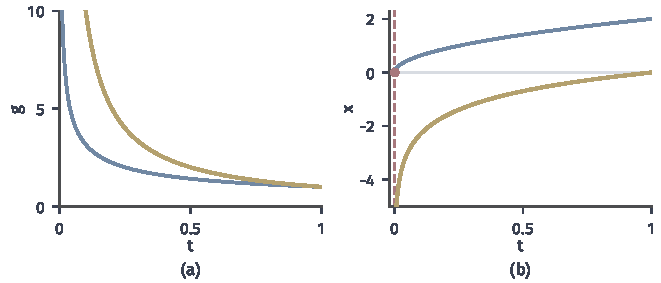
\includegraphics[width=112mm]{figures/06-differential-equations/01-ordinary-differential-equations/matplotlib/ivp-integrable-singular/figure.pdf}
 \caption{$t=0$处无界的输入。(a)$g=t^{-1/2}$（蓝）可积，$g=1/t$（黄）不可积。(b)蓝线是$\dot{x}=t^{-1/2}$，$x(0)=0$的解$2\sqrt{t}$；黄线是$\ln t$，当$t\downarrow 0$时发散，无法接到$t=0$（红色虚线）。}
 \label{fig:ivp-integrable-singular}
\end{BookInlineFigure}

这里只是检验给定曲线是否是解，并没有断言解一定存在。要保证存在，还需要右端对时间可测、对状态连续，并且在状态的紧集上被一个时间的可积函数控制；唯一性还需要状态方向上的局部Lipschitz系数对时间局部可积。这些条件和结论由第~\ref{chap:ode-existence-continuation}章给出。

\paragraph{时间方向与状态方向的不对称}
上面的不连续都在时间方向上。解穿过一个时间点只花一瞬间，那一点上右端的值不影响积分，所以时间方向的跳变是无害的。状态方向的跳变不同，解可能在跳变处长期停留，这时零测集的论证就失效了。

考虑$\dot{x}=-\sigma(x)$，$x(0)=0$，其中$\sigma(x)=1$（$x\geq 0$），$\sigma(x)=-1$（$x<0$）。这个方程在任何区间$[0,\varepsilon)$上都没有绝对连续解。

假设有解。若某时刻$t_1>0$有$x(t_1)>0$，取$t_2$为$t_1$之前$x$最后一次等于$0$的时刻。在$(t_2,t_1]$上$x>0$，方程给出$\dot{x}=-1$几乎处处成立，积分得$x(t_1)=-(t_1-t_2)<0$，矛盾。

若$x(t_1)<0$，同样取$t_2$，在$(t_2,t_1]$上$\dot{x}=+1$，积分得$x(t_1)=t_1-t_2>0$，也矛盾。所以$x\equiv 0$。但这时$\dot{x}=0$，而方程要求$\dot{x}=-\sigma(0)=-1$几乎处处成立，仍然矛盾。

这个反例说明，第~\ref{sec:ivp-state}节的扩充状态不能随便用来处理不连续的输入。把时间写成状态分量$s$之后，右端对$s$是不连续的，表面上成了“状态方向的跳变”。但因为$\dot{s}=1$，解以单位速度穿过$s$的每一个值，并不停留，所以这种不连续恰好无害。一般的状态方向的不连续不具备这个性质。假设中对时间只要求可测、对状态要求连续，分工的依据就在这里。

\paragraph{解的概念的层次}
图~\ref{fig:ivp-solution-classes}整理了本章出现的曲线类。越往外，允许的曲线越多，能用的输入越一般。绝对连续这一层的外面，曲线已经无法由导数累积回来，所以解的概念止步于此。

\begin{BookInlineFigure}
 \centering
 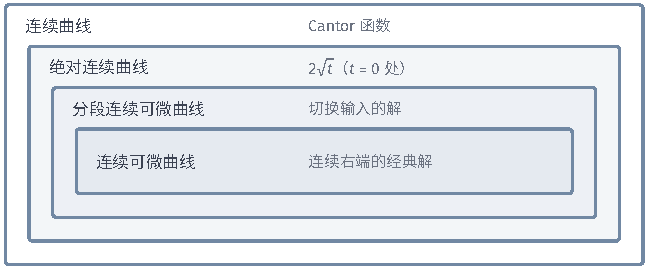
\includegraphics[width=109mm]{figures/06-differential-equations/01-ordinary-differential-equations/tikz/ivp-solution-classes/figure.pdf}
 \caption{本章涉及的曲线类，外层包含内层，右侧是每层的代表例子。连续右端的解在最内层，切换输入的解在第二层，可测输入的解在绝对连续这一层。Cantor函数只是连续，不能作为解。}
 \label{fig:ivp-solution-classes}
\end{BookInlineFigure}
